\documentclass[letterpaper,oneside,12pt]{book}

% Para asegurar compatibilidad en Windows y GNU/Linux
\usepackage[utf8]{inputenc}

% Idioma de entrada
\usepackage[spanish]{babel}

% Márgenes conforme a lo requerido en el reglamento de pregrado.
\usepackage[right=2cm,left=2.5cm,top=2.5cm,bottom=2.8cm,headsep=1cm,footskip=1.5cm]{geometry}

% Cabeceras y pie de página en páginas internas
\usepackage{fancyhdr}

% Para insertar gráficos, figuras y tablas
\usepackage{graphicx,tabularx,latexsym}

% Matemáticas avanzadas
\usepackage{amsthm,amsmath,amssymb,amsfonts}

\usepackage[hyperindex,colorlinks=true,linkcolor=blue,filecolor=blue,citecolor=blue,urlcolor=blue]{hyperref}
% \usepackage[final]{pdfpages}

% Para legras griegas en negrita.
\usepackage{bm}

% Fancy enumerate :P
\usepackage{enumerate}

% Para poder usar acrónimos
\usepackage{acronym}

% Para tener subfiguras
\usepackage{subfigure}

% ***********************************************************************************
% ***********************************************************************************
\begin{document}


% ***********************************************************************************
% Redefinir nombres conforme reglamento de pregrado.
\renewcommand{\contentsname}{Índice General}
\renewcommand{\figurename}{\textbf{Fig.}}
\renewcommand{\tablename}{\textbf{Tabla}}
\renewcommand{\listfigurename}{Índice de Figuras}
\renewcommand{\listtablename}{Índice de Tablas}
%\renewcommand{\listofacronyms}{Índice de Acrónimos}

% Redefinir espaciado simple a 1.5, conforme a reglamento.
\renewcommand{\baselinestretch}{1.5}

% Los capítulos se trabajan en forma independiente para no tener un solo archivo .tex sobrecargado con información. Luego cada uno de los archivos se inserta en el archivo global mediante el comando \input{}. Uno de los mejores puntos de esta forma de trabajar es que se pueden realizar cambios en algunas partes sin perder la información de todo el documento.

% ***********************************************************************************
% PORTADA
\thispagestyle{empty}

\includegraphics[width=1.5cm]{Figures/Escudo}
\put(10,38){UNIVERSIDAD DE CONCEPCIÓN0}
\put(10,23){FACULTAD DE INGENIERÍA}
\put(10,8){DEPARTAMENTO DE INGENIERÍA ELÉCTRICA}


\vspace{0.3cm}
\large
\begin{flushright}
\textbf{Prof. Patrocinante:}\\
Nombre Profesor, Grado académico.
\end{flushright}

\vspace{3.5cm}
\begin{center}
\LARGE \textbf{Posicionamiento indoor mediante seguimiento de interfaces de red de equipos móviles.}\\

\vspace{1cm}
\Large \textbf{Aldo Nicolás Mellado Opazo}

\vspace{0.9cm}
Informe de Memoria de Título para optar al Título de \\Ingeniero Civil en Telecomunicaciones

\vspace{2.5cm}
Concepción, Chile. \\
\today
\end{center}
\normalsize

% ***********************************************************************************
% RESUMEN
\newpage 
\pagestyle{plain}	% Para no tener encabezado
\pagenumbering{roman}	% Para numerar en forma romana, i.e. I, II, III, etc.
\chapter*{Resumen}

La historia nos dice que conforme evolucionan la especies lo hacen sus necesidades. En un comienzo el humano nómada necesitaba alimento y cobijo y debido a esto, se adaptó a sus necesidades, años mas tarde con la agricultura y la domesticación precindió de moverse de un lugar a otro para las necesidades básicas e hizo que el entorno se adaptara a sus requerimientos, sin embargo, al evolucionar el colectivo y por tanto, las estructuras políticas y sociales el ser humano tuvo que movilizarse, viajar, recorrer nuevos terrenos y para ello requirió de herramientas; mapas, cartas de navegación y más tarde, radares.

En la actualidad, para satisfacer nuevas y complejas necesidades hemos creado sofisticadas y novedosas herramientas para guiarnos, las cuales nos permiten, entre otras cosas llegar de una ciudad a otra, encontrar un local de comida al otro lado de la cuidad y ahorrarnos el tráfico movilizandonos por la ruta más óptima, una que nos ahorre el tráfico o tediosos pagos de peaje. Todo esto y más ha sido resuelto con la implementación de algoritmos en aplicaciones móviles que nos permiten hacer todo lo anteriormente mencionado.\\

Los algoritmos usados en espacios exteriores se valen del \ac{GPS}, sin embargo, este sistema resulta, dada la precisión de sus mediciones poco eficiente a la hora de determinar la posición en un espacio interior, esto pues la señal del satélite no es capaz de atravesar los muros y otras superficies, y es por este motivo que se quiere implementar un sistema que resuelva las nuevas necesidades que se presentan en los espacios indoor y para lo cual se requiere utilizar \ac{IPS}.\\

\addcontentsline{toc}{chapter}{Resumen} % Para agregar el resumen al índice como un capítulo más, pero sin número.

% ***********************************************************************************
% INDICE GENERAL: Requerido por reglamento
\newpage
\tableofcontents

% INDICE DE FIGURAS: No es requerido, pero se agradece por facilitar corrección

%\newpage
%\listoffigures
%\addcontentsline{toc}{chapter}{\listfigurename}

% % INDICE DE TABLAS: No es requerido, pero se agradece por facilitar corrección
%\newpage
%\listoftables
%\addcontentsline{toc}{chapter}{\listtablename}

\newpage
\chapter*{Lista de Acrónimos}
%\listofacronyms
%\addcontentsline{toc}{chapter}{\listofacronyms}
\addcontentsline{toc}{chapter}{Índice de Acrónimos}
% ***********************************************************************************
% Acronym definitions

\acrodefplural{AP}[AP's]{Access Points}


\begin{acronym}
\acro{GPS}{Global Positioning System}   	
\acro{WiFi}{Wireless Fidelity}
\acro{AP}{Access Point}
\acro{IPS}{Indoor Positioning System}
\acro{RSS}{Received Signal Strength}
\acro{AOA}{Angle of Arrival}
\acro{TOA}{Time of Arrival}
\acro{MAC}{Media Access Control}

\end{acronym}

% ***********************************************************************************
% ***********************************************************************************
%\newpage
%\chapter*{Agradecimientos}

Acá van los agracedimientos. Es la única parte que se acepta como informal, por lo que depende de cada alumno si quiere dar gracias.

\vspace{0.2cm}
A todos uds. gracias.

\vspace{1cm}
Sinceramente,
\begin{flushright}
 \textbf{Nombre del Alumno}
\end{flushright}



%\addcontentsline{toc}{chapter}{Agradecimientos}
%

% ***********************************************************************************
\newpage
\pagestyle{fancy} 	% Se introduce la cabecera previamente definida
\pagenumbering{arabic}	% Se numera de forma normal.
% ***********************************************************************************
% ---------------------            INTRODUCCIÓN                 ---------------------
% ***********************************************************************************
\chapter{Introducción}

% ***********************************************************************************
% ***********************************************************************************
\section{Antecedentes Históricos}

En la década de los 60's el Departamento de Defensa de los Estados Unidos desarrolló el primer prototipo de un sistema de geolocalización basado en el cálculo de la diferencia de fases de la señales emitidas desde un satélite a estaciones terrestres, lo que les permitía determinar su posición. Años más tarde, en la década de los 70's los programas de la armada y de la Fuerza Aérea desarrollaron un sistema mejorado que les permitía determinar posiciones en el planeta mediante el uso de 24 satélites dispuestos a 20.200 km.\\

Mediante el uso de un método matemático llamado Trilateración, son capaces de usar los satélites y la cobertura estos hacen sobre la superficie de la tierra, para comparar la posición del dispositivo, con otras 3 unidades fijas de distancia. Las mediciones y la cobertura de este sistema se hace más exacta conforme se cubren más áreas, de ahí la necesidad de 24 satélites.\\

Sin embargo, dicho método no aplica para espacios indoor y es allí donde aparecen prototipos de GPS para indoors, también llamados Sistemas de Posicionamiento Indoor (\ac{IPS}) en los que implementaciones como las hechas por Google que, tras añadir a su aplicación Google Maps planos de pisos en centros comerciales, aeropuertos y otras grandes áreas comerciales, permiten al usuario moverse estando en conocimiento de accesos, salidas de emergencia y ubicaciones de tiendas. 


% ***********************************************************************************
% ***********************************************************************************
\section{Definición del Problema}

Para personas con algún tipo de discapacidad es de por sí muy tedioso y dificil hallar un lugar en el estacionamiento, encontrar un acceso habilitado para sillas de ruedas, ascensores y baños, especialmente si se trata de algún usuario que se halla de paso en la ciudad.\\

Además de lo anterior, es sabido que para las tiendas de retail es importante poder concentrar de mejor manera sus esfuerzos para captar clientes y comprender el comportamiento basado en el interés que estos muestran por determinados productos y la forma en que la disposición de estos influye en sus hábitos de compra.\\

Todo esto se puede lograr diseñando un sistema de posicionamiento indoor que entregue una ubicación exacta al usuario, ya sea para encontrar accesos y facilitar la navegación de este al interior de un centro comercial, de un hospital o para guiar un robot, para hallar un vehículo en un estacionamiento subterráneo o para entregar informes sobre comportamientos de clientes en una tienda en particular.\\

La utilidad y aplicabilidad de este sistema incuestionable\footnote{https://www.prnewswire.com/news-releases/indoor-positioning-and-navigation-system-market-to-provide-over-usd-25-billion-revenue-post-2016-300362071.html} y es por ello que urge una implementación que de respuesta a esta oportunidad.

% ***********************************************************************************
% ***********************************************************************************
\section{Estado del Arte}

En la actualidad existen diversos algoritmos de posicionamiento indoor basados en el uso de redes Wifi, no obstante, pueden ser clasificados en categorías según el tipo de enfoque que tienen estos: Algoritmo de proximidad, algoritmo de triangulación y algoritmo de análisis de ambiente.



% ***********************************************************************************
% ***********************************************************************************
\section{Hipótesis de Trabajo}
En lenguaje coloquial, es con lo que uno se ``compromete''.

% ***********************************************************************************
% ***********************************************************************************
\section{Objetivos}
% ***********************************************************************************
\subsection{Objetivo General}


% ***********************************************************************************
\subsection{Objetivos Específicos}
\begin{itemize}
 \item Objetivo 1
 \item Objetivo 2
 \item Objevivo 3..
\end{itemize}

% ***********************************************************************************
% ***********************************************************************************
\section{Alcances y Limitaciones}
Aquí se indican los aportes mayores realizados por este trabajo y se indican claramente las limitaciones asumidas.

En general las limitaciones se dejan planteadas a resolver en el trabajo futuro.


% ***********************************************************************************
% ***********************************************************************************
\section{Temario y Metodología}
Se hace una pequeña descripción del contenido de cada capítulo.

 
% ***********************************************************************************
\newpage
\chapter{Marco Teórico}
% ***********************************************************************************

En el proceso de comunicación se tiene que además del emisor, el receptor y el mensaje, existe el canal, el cual para la propagación de las ondas electromagnéticas corresponden al aire o bien, a un cable conductor. Estas son usadas para transmitir información en forma de señales que en comunicaciones, viajan por distintos medios, cables de cobre, fibra óptica o enlaces de microondas, entre otros.\\

Sin embargo, la información, considerando el volumen de datos que viajan por las redes, obedece un orden, que en redes de datos se conoce como modelo OSI.\\

\section{Modelo OSI}

Es un modelo que sirve de referencia para los protocolos que operan en las distintas capas que componen este modelo. Es un estándar desarrollado en 1980 por la ISO que establece un ordenamiento por el cual deben regirse los datos al moverse.\\

\newpage
\underline{Este modelo consta de siete capas}\\

Físico, Enlace, Red, Transporte, Sesión, Presentación, Aplicación.

Donde cada nivel realiza una función concreta, y se separa de los adyacentes por interfaces conocidas, sin que le concierna ningún otro aspecto del total de la comunicación.  Las capas que participan de los modelos estudiados son las que se detallan a continuación:

\subsection{Capa Física}

Corresponde a las capa que guarda relación con la conexión, es decir, con la forma en que se conecta el dispositivo a la red y la transmisión, esto es a cómo se transmiten los datos. Entre sus funciones, está el establecer cuál o cuáles son los medios por los cuales viaja la señal y el normar las características materiales y eléctricas de los componentes.\\

\subsection{Capa de Enlace}
Esta capa representa para efectos de lo que se pretende investigar y eventualmente desarrollar, la capa que hace posible el seguimiento, pues se encarga de la transferencia de información entre la capa de red y la capa física. Y para ello se vale de tramas que le dotan al dispositivo una dirección \ac{MAC} lo que le permite hacer control de flujo, detección y corrección de errores.\\

Es de esta capa que los IPS, se valen, como es el caso de el algoritmo de trilateración en donde se establece la conexión a un AP, se hace la identificación del dispositivo a través de la dirección MAC y luego el posterior cálculo.

\section{Medio No Guiado}

Corresponde a los medios por los cual viajan las ondas electromagnéticas y que en este caso, corresponden a dispositivos que se valen de antenas para propagarlas.

\section{Router}

Un router inalámbrico es un dispositivo que además de la función de router, sirve de punto de acceso, es decir, permite que los dispositivos inalámbricos se conecten a la red. En las funciones de router, este dispositivo direcciona los datos que provienen desde y hacia los dispositivos conectados a la red y que compartan la misma conexión de red por las distintas interfaces que la compongan, permitiendo que estos se comuniquen entre sí.\\

Todas las conexiones realizadas en la red inalámbrica se hacen dentro de lo que se denomina, para cuando se usa este tipo de redes, una red de infraestructura inalámbrica y es sobre esta que los dispositivos se comunican entre si e interactúan con la red exterior.\\

Es en esta parte donde el router recibe, desde el dispositivo móvil, solicitudes del tipo \textsc{ICMPv6}, que son un tipo de solicitudes conocidas como \ac{IRDP}  o Protocolo de descubrimiento de enrutador de internet y que son un tipo de solicitudes del protocolo \ac{ICMP} o Protocolo de control de mensajes de internet que se encargan de establecer la conexión con el router. Del tipo de mensajes ICMP existen dos tipos:\\

\begin{itemize}
\item{\textit{ICMP Router Solicitation Message:} Este tipo de mensajes es enviado desde un equipo a cualquiera de los routers que se hallen en la LAN para avisar que se encuentran en presencia de esta red. Básicamente, avisan que podrían eventualmente desear conectarse.}
\item{\textit{ICMP Router Advertisement Message}: Es enviado por el router en la LAN para anunciar la IP disponible para rutear.}\\
\end{itemize}

\begin{figure}[h!]
\centering
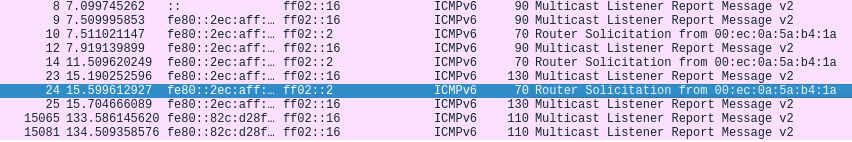
\includegraphics[scale=0.5]{./imagenes/IRDP}
\caption{Captura en Wireshark de solicitudes IRDP}
\label{fig:IRDP}
\end{figure}

Finalmente, se anuncian mediante una solicitud de establecimiento de conexión donde el router recibe la MAC del dispositivo, entre otros datos, y establece la conexión si la autenticación fue exitosa.\\


\begin{figure}[h!]
\centering
		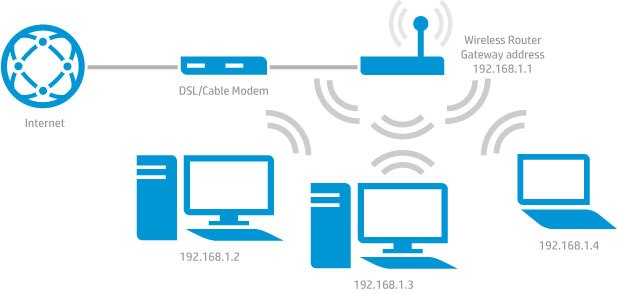
\includegraphics[scale=0.5]{./imagenes/ap}
		\label{fig:access_point}
		\caption{Ejemplo de red de infraestructura inalámbrica$^{\ref{fig:paginaHP}}$}
\end{figure}

De ser exitosa, el router, mediante el protocolo \ac{DHCP}, asigna desde el número limitado de direcciones IP que el \ac{ISP} entrega al cliente, una IP que enlaza esta dirección con la MAC del usuario estableciendo así la conexión. Es así como del router inalámbrico el dispositivo posee ahora la conexión al AP WiFi.

\section{Wifi}

Es una tecnología que recibe su nombre a partir de la abreviación de una marca comercial y que permite el acceso a la red por parte de dispositivos de forma inalámbrica, haciendo así posible  la vinculación de diferentes equipos entre si prescindiendo de cables.\\

Dado que la conexión inalámbrica se hace a través de ondas electromagnéticas dentro del rango de frecuencias en los 2.4 GHz y que estas se dividen en 14 canales que van desde los 2412 MHz hasta los 2484 MHz, existen combinaciones óptimas de canales en las que estos no se solapan entre si, y con ello, se logran reducir las interferencias.\\

Esta tecnología está regulada por el estándar internacional IEEE 802.11 que con el paso del tiempo, ha dado lugar a otras versiones que incluyen mejoras tales como ancho de banda, alcance, velocidad y frecuencia.\\

Para efectos de este estudio, se deben tener en consideración las pérdidas propias de la propagación de estas ondas. Ejemplo de la propagación de la señal de Wifi en un espacio es el presentado en la imagen \ref{fig:propagacion} \\

\begin{figure}[h!]
\centering
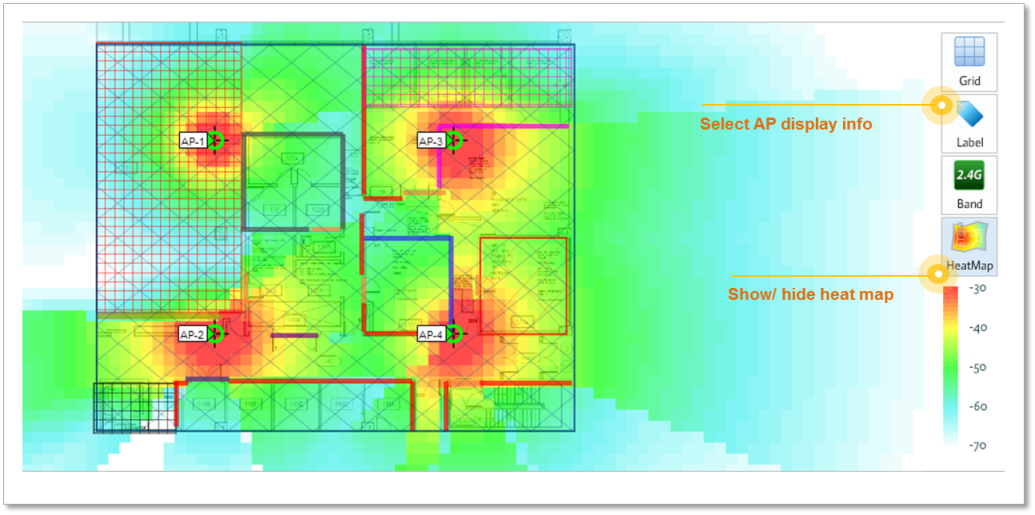
\includegraphics[scale=0.8]{./imagenes/propagacion}
\caption{Muestra software D-link sobre variación de intensidad de señal por propagación en espacio indoor.$^{\ref{fig:prop}}$}
\label{fig:propagacion}
\end{figure}

\newpage 

\section{Modelo de propagación}

Son aproximaciones matemáticas que permiten modelar el espacio físico por el cual se va a propagar la señal y que contemplan los principios físicos que la describen y que se introducen al modelo en forma de parámetros. Y que para efectos de este estudio, permiten caracterizar los valores esperados según el tipo de espacio que se vaya a caracterizar para así tener un marco de referencia con el cual contrastar las mediciones obtenidas.\\

\textit{''Estos modelos a menudo se basan en modelos probabilísticos, que pueden calcular con una cierta probabilidad de que la señal llegue o no a un determinado lugar. Algunos de estos modelos se basan en mediciones realizadas en el lugar de interés de las cuales se toman miles de mediciones que se promedian, pudiendo entonces, establecerse modelos de propagación en estos medios''} \ref{pdf:modprop}. De esta forma, cada modelo sirve para cada entorno, pudiendo estos a su vez, servir de base para otros modelos. Es por esto que se trabaja apoyándose tanto de información estadística como de teorías matemáticas.\\

Dado que el espacio a caracterizar, para el uso de IPS, se trata de espacios interiores, se tiene que los modelos de este tipo a aplicarse serían:\\

\subsection{Modelo de propagación Indoor}

Corresponden a un tipo de modelo de propagación que se adecúa a la forma en que se propagan las ondas en un espacio indoor. Contemplan fenómenos físicos como son la reflexión, la refracción y la atenuación. Estudian además, cuáles son las variantes que se adecúan mejor al espacio, es decir, si se trata de un espacio físico de varios 
pisos o de una sola planta.\\

\subsection{Modelo de propagación en espacio libre - Ecuación de FRIIS:} 

El modelo de propagación en espacio libre, es utilizado para estimar el nivel de potencia que se recibiría en determinado lugar cuando no se está en presencia de objetos que puedan degradar la señal, afectando la propagación de esta entre el transmisor y el receptor. Esta condición es conocida como \ac{LOS} o línea de vista.\\

Pese a lo estricto que es el tener que considerar que la señal no se propagará en un entorno con obstáculos, el modelo FRIIS es una buena referencia de comparación para enlaces de mayor complejidad. Este modelo establece que el decaimiento de la potencia es una función que depende de la distancia de separación entre el transmisor y el receptor, elevada a alguna potencia.\\

Dicha relación queda de manifiesto en la siguiente ecuación.

\begin{equation}
PL = 10\cdot{log{\left(\dfrac{P_t}{P_r}\right)}} = -10\cdot{log\left(\dfrac{\lambda^2}{(4\pi)^2\cdot{d^2}}\right)}\\
\end{equation}

donde\\

\begin{itemize}
\item{$P_t$: es la potencia transmitida, en este caso, por el router}
\item{$P_r$: es la potencia recibida, en este caso, por el equipo}
\item{$\lambda$: Es la longitud de onda a la que opera, en este caso, Wifi}
\item{$d$: Representa la distancia a la que se realiza la medición.}
\end{itemize}

De lo anterior, se tiene que la ecuación de Friis muestra, como la potencia de la señal recibida, se atenúa de acuerdo al cuadrado de la distancia entre el transmisor y el receptor. \\

\subsection{Linear Path Attenuation Model} 

Es un modelo que se usa para cuando el transmisor y el receptor se hallan en la misma planta. Las pérdidas por propagación están en dB y se obtienen a partir del \textit{path loss} en espacio libre, $PL_{FS}$, además de un factor que es lineal y que se obtiene experimentalmente.\\

Este modelo se vale de la siguiente fórmula:

\begin{equation}
PL(d) =  PL_{FS} + a\cdot{d}
\end{equation}

Donde $a$ es el coeficiente de atenuación lineal, y $d$ es la distancia entre Tx y Rx. Este coeficiente obedece a datos tabulados según el ambiente en el que se hizo la medición y que para el caso de oficinas sería de 0.47 dB/m. 


\subsection{Modelos basados en Redes Neuronales (ANNs)}{\label{redesneuronales}}

Este tipo de modelos, recoge las imprecisiones de modelos tales como los empíricos, donde la falta de precisión es la principal deficiencia, y de modelos deterministas que si bien otorgan precisión, son altamente ineficientes, puesto que a menudo, requieren altas capacidades de procesamiento, y basándose en redes neuronales que aprovechan una base de datos de la planta en que se desea implementar, permiten con gran rapidez llegar a resultados precisos. \\

Dicha base de datos se compone de datos sobre zonas compuestas de diferentes categorías de materiales, superficies y objetos que existen en el entorno, además de la distancia entre el transmisor y el posible receptor, debiendo además, incluir información sobre el número y el tipo de materiales con que se va a encontrar la señal en las distintas categorías.\\

Las ANNs además de precisión, se valen del paralelismo sobre el cual se implementan proveyendo así una rápida evaluación de los resultados, y donde si bien, los procesos de aprendizaje suelen ser del orden de las horas, los procesos que le suceden en la predicción de niveles, es rápido.


% ***********************************************************************************
%\newpage
%\chapter{Revisión Bibliográfica}
% ***********************************************************************************
\section{Introducción}
En este capítulo se hará una revisión de los textos consultados en el desarrollo de este estudio, ahondando en los elementos que estos aportan al definir, de entre todos los métodos, modelos y técnicas de posicionamiento Indoor.\\
% ***********************************************************************************
\subsection{Recent Advances in Wireless Indoor Localization Techniques and System}
\subsubsection{Abstract}

\emph{Los avances en las tecnologías basadas en la localización y la creciente importancia de la informática ubicua y la información dependiente del contexto han llevado a un creciente interés comercial en aplicaciones y servicios basados en la ubicación. En la actualidad, la mayoría de los requisitos de las aplicaciones son la localización o el seguimiento en tiempo real de las pertenencias físicas dentro de los edificios con precisión; por lo tanto, la demanda de servicios de localización en interiores se ha convertido en un requisito previo clave en algunos mercados. Además, las tecnologías de localización de interiores abordan la inadecuación del sistema de posicionamiento global dentro de un entorno cerrado, como los edificios. Sin embargo, sobre la base de esto, este documento tiene como objetivo proporcionar al lector una revisión de los avances recientes en técnicas y sistemas de localización de interiores inalámbricos para ofrecer una mejor comprensión del estado del arte de tecnologías y motivar nuevos esfuerzos de investigación en este campo prometedor. Para este propósito, se revisan los sistemas existentes de localización inalámbrica y los esquemas de estimación de ubicación, ya que también comparamos las técnicas y sistemas relacionados con una conclusión y trabajos futuros.}\\

Este documento hace una revisión acabada de los distintos métodos empleados en el desarrollo de sistemas de posicionamiento indoor comparando las ventajas y desventajas entre ellos. Es especialmente útil pues permite entender porqué es que se usan preferentemente métodos asociados a variables que no dependan tanto de la potencia, sino que a variables relacionadas con la propagación de la señal en estos espacios. Es así que se descartan métodos tales  como el de proximidad, aún cuando este tiene un costo computacional bajo, para escoger métodos  relacionados con el ToA, donde se prioriza la exactitud por sobre el costo computacional. Además, se mencionan otros métodos tales como, Map Matching, el cual es un algoritmo basado en algoritmos de proyección y reconocimiento de patrones.\\

Sin embargo, es finalmente la capacidad computacional, así como la inmediatez con la que se necesitan los resultados, lo que sugiere que métodos de bajo requerimiento computacional sean candidatos óptimos.

\subsection{WIFI-Based Indoor Positioning System}
\subsubsection{Abstract}

\emph{El fácil acceso y la disponibilidad de las tecnologías inalámbricas y la informática móvil e Internet han dado lugar a nuevas oportunidades en el desarrollo de aplicaciones móviles cuyo propósito es facilitar la vida de las personas. Hoy en día, una persona puede poseer más de un dispositivo móvil para diferentes usos, como comunicación, entretenimiento, trabajos de oficina. Este documento propone una aplicación móvil que podrá estimar la posición de un usuario dentro de un edificio mediante el uso de la tecnología WIFI.}\\

Este texto plantea que dentro de las posibilidades de desarrollo que se han abordado para poder llegar a implementar un sistema de posicionamiento indoor, han sido consideradas varias tecnologías entre las cuales están; bluetooth, Wifi, RFID e incluso Infrarrojo. Sin embargo, comenta que dada la penetración que ha tenido la tecnología Wifi en ambientes indoor este ha sido elegido por sobre los otros, dejando así, una amplia oportunidad de desarrollo basada en las propiedades de funcionamiento, dado que no requiere invertir en hardware especializado. Razón por la cual se valida usar en este estudio, a Wifi como la tecnología apropiada.\\

Además, este paper introduce nociones sobre lo que es la detección de \ac{RSS} desde los distintos AP disponibles y que, basados en la asociación de las distintas posiciones recibidas e informadas a la dirección MAC, se puede hacer un seguimiento de los dispositivos basándose en la potencia informada y la MAC. Se apoya además de una base de datos que consiste en los niveles de potencia recibidos y almacenados en un vector que caracteriza el espacio, y se complementa con la distancia euclidiana que, como plantean el documento <<\textit{es usada para comparar la posición obtenida actual en la aplicación móvil y la posición almacenada en la base de datos en el servidor.}>>

\subsection{A Comparison of algorithms adopted in figerprint indoor positioning systems}
\subsubsection{Abstract}

\emph{La tecnología de huellas digitales se ha utilizado ampliamente en sistemas de posicionamiento en interiores como los sistemas de posicionamiento Wi-Fi. Su desempeño depende no sólo de la medición de la intensidad de la señal, sino que también del algoritmo utilizado. En este documento, da una visión general de los algoritmos populares actuales adoptados en sistemas de posicionamiento indoor basados en WIFI, incluido el método determinista (K vecino más cercano, K peso vecino más cercano), método probabilístico y red neuronal. En orden para obtener un resultado confiable y representativo, esos algoritmos se evalúan en función en la misma base de datos Se hicieron comparaciones con respecto al posicionamiento precisión, complejidad computacional y el tamaño de la base de datos. Además, los detalles de elección de parámetros y la implementación de estos algoritmos son discutido.}\\

Este texto sirve de apoyo para lo que se planteó en el marco teórico, puntualmente en el item de métodos de estimación de posición basado en Redes Neuronales \ref{redesneuronales}, pues realiza una comparación entre la eficiencia, la calidad, cantidad y naturaleza de los parámetros que se obtienen, decretándose que para el caso de las redes neuronales, si bien se conserva la idea de recabar información desde los niveles de potencia recibidos,  se requiere de un entrenamiento previo tedioso, lento y de alto consumo computacional. Razón por la cual, al requerirse para el tipo de espacio, ambiente y potencial cliente respuestas rápidas las redes neuronales no son una alternativa en el corto plazo.\\

Además, el texto hace una comparación entre otros métodos de estimación de posición basándose en técnicas que se apoyan de la \ac{RSS} y aquellos basados en propiedades geométricas. Del texto se extrae de mejor manera la noción de qué tipo de método debería escogerse, si uno probabilístico o uno empírico.

\subsection{Wi-Fi In-door Positioning System Based on RSSI Measurements from Wi-Fi Access Points - A Tri-lateration Approach}
\subsubsection{Abstract}	
%Positioning is the most attractive technology today. Various technologies are used now days for positioning purpose. GPS is mainly used for outdoor environment. Non-suitability of GPS in indoor conditions because of its NLOS conditions and signal attenuation has lead to several other techniques of indoor positioning. This paper compares few indoor positioning methods and proposes indoor positioning system using tri-lateration method which uses RSSI data from wi-fi access points to do localization in indoor environment.\\

\emph{El posicionamiento es la tecnología más atractiva hoy en día. Varias tecnologías se utilizan ahora días para el propósito de posicionamiento. El GPS se usa principalmente para entornos al aire libre. La no idoneidad del GPS en interiores debido a sus condiciones NLOS y la atenuación de la señal ha llevado a varias otras técnicas de posicionamiento en interiores. Este documento compara pocos métodos de posicionamiento en interiores y propone un sistema de posicionamiento en el interior que utiliza un método de trilateración que utiliza datos RSSI de los puntos de acceso wi-fi para hacer la localización en el ambiente interior.}\\

Además de los métodos basados en parámetros no relacionados con la potencia, existen aquellos que combinan propiedades geométricas y nociones implementadas en tecnologías predecesoras a los IPS, para dar como resultado un método de trilateración que experimentalmente demuestra tener resultados de calidad mas bien baja, y que si bien, los resultados permiten estimar la posición, distan considerablemente del resultado que se persigue en este estudio, mas entregan un marco de referencia, tanto en conocimientos teóricos y de resultados experimentales que ciertamente serán de utilidad a la hora de optar por un método u otro.


\subsection{WIFI-based indoor positioning system}
\subsubsection{Abstract}	
%Recently, several indoor localization solutions based on WiFi, Bluetooth, and UWB have been proposed. Due to the limitation and complexity of the indoor environment, the solution to achieve a low-cost and accurate positioning system remains open. This article presents a WiFi- based positioning technique that can improve the localization performance from the bottle- neck in ToA/AoA. Unlike the traditional approaches, our proposed mechanism relaxes 
%the need for wide signal bandwidth and large numbers of antennas by utilizing the transmis- sion of multiple predefined messages while maintaining high-accuracy performance. The overall system structure is demonstrated by showing localization performance with respect to different numbers of messages used in 20/40 MHz bandwidth WiFi APs. Simulation resultsshow that our WiFi-based positioning approach can achieve 1 m accuracy without any hardware change incommercial WiFi products, which is much better than the conventional solutions from both academia and industry concerning the trade-off of cost and system complexit.

\emph{Recientemente, se han propuesto varias soluciones de localización de interiores basadas en WiFi, Bluetooth y UWB. Debido a la limitación y complejidad del entorno interior, la solución para lograr un sistema de posicionamiento preciso y de bajo costo permanece abierta. Este artículo presenta una técnica de posicionamiento WiFibased que puede mejorar el rendimiento de localización del cuello de botella en ToA / AoA. A diferencia de los enfoques tradicionales, nuestro mecanismo propuesto relaja la necesidad de un amplio ancho de banda de señal y un gran número de antenas al utilizar la transmisión de múltiples mensajes predefinidos mientras se mantiene el rendimiento de alta precisión. La estructura general del sistema se demuestra al mostrar el rendimiento de localización con respecto a los diferentes números de mensajes utilizados en los AP WiFi de banda ancha de 20/40 MHz. Los resultados de simulación muestran que nuestro enfoque de posicionamiento basado en WiFi puede alcanzar 1 m de precisión sin ningún cambio de hardware en productos WiFi comerciales, que es mucho mejor que las soluciones convencionales de la academia y la industria en relación con el costo y la complejidad del sistema.}\\

La utilidad de este documento reside en la información que entrega respecto de la calidad y naturaleza de los parámetros utilizados, donde a diferencia de otros documentos consultados, este presenta variables que no se apoyan sólo de métodos geométricos, ni basados en la intensidad de potencia recibida, sino que entregan herramientas tales como el \ac{TOA}, el \ac{AOA} y un híbrido entre los dos anteriores. La calidad y claridad de los conceptos que entregan permite comprender porqué, como se ha señalado en documentos anteriores, estos parámetros de no ser que estos requieren un alto consumo computacional, serían la base de los IPS. Presenta en este estudio, procedimientos probabilísticos para dotar de mayor precisión a la estimación, herramientas basadas en análisis espectrales de las señales recibidas y que relacionan la fase.

%\subsection{Mobile indoor positioning using Wifi localization and image processing}
%\subsubsection{Abstract}	
%%At present, there has been an increased interest in indoor positioning systems that propelled researchers to come up with various solutions. A number of these research either use Wi-fi Localization or image processing; each having problems with either accuracy or speed. In this paper, we propose a framework which will use both Wi-fi Localization and image processing to address this problem. The framework used Wi-fi Localization to calculate the estimated position of the user then refine the accuracy through image processing. The designed framework was able to surpass the performance of Wi-fi Localization algorithms in accuracy, and image processing in speed. Different techniques were also applied that improved accuracy and made the system calculate for the location faster.
%
%\emph{En la actualidad, ha aumentado el interés en los sistemas de posicionamiento en interiores que impulsaron a los investigadores a encontrar varias soluciones. Algunas de estas investigaciones utilizan la localización Wi-Fi o el procesamiento de imágenes; cada uno tiene problemas con la precisión o la velocidad. En este documento, proponemos un marco que utilizará tanto la localización Wi-Fi como el procesamiento de imágenes para abordar este problema. El marco utilizó la localización Wi-Fi para calcular la posición estimada del usuario y luego refinar la precisión mediante el procesamiento de imágenes. El marco diseñado fue capaz de superar el rendimiento de los algoritmos de localización de Wi-Fi en precisión, y el procesamiento de imágenes en velocidad. También se aplicaron diferentes técnicas que mejoraron la precisión e hicieron que el sistema calculara la ubicación más rápido.}


\subsection{Mobile indoor positioning using Wifi localization}
\subsubsection{Abstract}
\emph{El objetivo de este documento es crear una aplicación que describa el método de trilateración Wi-Fi para el posicionamiento en interiores utilizando dispositivos móviles basados en Android. Los objetivos, alcances, limitaciones y la importancia de esta investigación también son temas tratados en este artículo. El problema de propagación de la señal interior se resuelve al recibir una colección de medidas de intensidad de la señal que mejora la precisión de la localización. El tema de precisión implica el conocido problema de la propagación de la señal en interiores que se resuelve mediante la recopilación de mediciones de la intensidad de la señal recibida y su uso en el algoritmo de trilateración. La técnica de posicionamiento en interiores abre posibilidades para el desarrollo de varios sistemas inteligentes que proporcionan al usuario información basada en la ubicación dentro de los edificios.}\\

El aporte de este documento recae en la presentación de una implementación en un sistema operativo android de lo que puede ser un sistema de posicionamiento, plantea que usando el método geométrico de trilateración es posible estimar la posición basándose en la potencia informada por el usuario, lo que permitiría, a través de esta misma aplicación darle a conocer a un usuario su ubicación. Mas dista de ser lo que persigue este estudio dado que si bien resuelve el posicionamiento, es pobremente aplicable a un sistema de seguimiento o de posicionamiento en tiempo real.

\subsection{An Improved WiFi Indoor Positioning Algorithm by Weighted Fusion}
\subsubsection{Abstract}
\emph{El rápido desarrollo de Internet móvil ha brindado la oportunidad de que el posicionamiento en interiores de WiFi pase a ser el centro de atención debido a su bajo costo. Sin embargo, hoy en día la precisión del posicionamiento WiFi en interiores no puede satisfacer las demandas de aplicaciones prácticas. Para resolver este problema, este documento propone un algoritmo de posicionamiento de WiFi mejorado mediante fusión ponderada. El algoritmo propuesto se basa en los algoritmos tradicionales de huellas digitales de ubicación y consta de dos etapas: la adquisición fuera de línea y el posicionamiento en línea. El proceso de adquisición fuera de línea selecciona los parámetros óptimos para completar la adquisición de la señal, y forma una base de datos de huellas dactilares por clasificación y manejo de errores. Para mejorar aún más la precisión del posicionamiento, el proceso de posicionamiento en línea primero usa un método previo al partido para seleccionar las huellas dactilares candidatas para acortar el tiempo de posicionamiento. Después de eso, utiliza la distancia euclidiana mejorada y la probabilidad conjunta mejorada para calcular dos resultados intermedios, y calcula además el resultado final de estos dos resultados intermedios por fusión ponderada. La distancia Euclidiana mejorada introduce la desviación estándar de la intensidad de la señal WiFi para suavizar la fluctuación de la señal WiFi y la probabilidad conjunta mejorada introduce el cálculo logarítmico para reducir la diferencia entre los valores de probabilidad. Comparando el algoritmo propuesto, el algoritmo euclidiano WKNN basado en la distancia y el algoritmo de probabilidad conjunta, los resultados experimentales indican que el algoritmo propuesto tiene una mayor precisión de posicionamiento}\\

Dentro de los documentos consultados, donde se han expuesto métodos basados en potencia, en propiedades geométricas y en el conocimiento claro de la ubicación de los AP, aparece lo que expone el autor, donde además de presentar conceptos esenciales relacionados con los distintos métodos de cálculo de la posición en los que se basa la implementación de los IPS, aparece también la idea de realizar posicionamiento indoor prescindiendo de conocer la ubicación de los APs. Señala que dentro de los problemas que existen a la hora de implementar un sistema, está el hecho de que generalmente no se conocen los APs dispuestos en otros espacios o por otros clientes y además, que la precisión de los métodos presentados anteriormente es mas bien cuestionable debido a ser poco adecuada a los ambientes que se desea implementar.\\

Plantea la necesidad de incluir en el método, un entrenamiento previo, que básicamente recoge los niveles de potencia recibidos en el área de estudio, la cual es previamente dividida en sectores equidistantes y asociar estos niveles al sector en que se halla el usuario. Corrige impresiciones en las mediciones mediante la inclusión de otros parámetros tales como la potencia promedio, la desviación estándar y  el valor promedio de la potencia procesada. Lo destacable de este documento es que expone la posibilidad de estimar la posición del usuario sin tener que conocer la ubicación de los APs.

\subsection{Characterizing Wi-Fi Network Discovery}
\subsubsection{Abstract}
%In the Wi-Fi network discovery phase, the probe request sent by a mobile device is not encrypted. Therefore, the MAC address contained in the probe request frame can be exploited to track users without their knowledge and consent. To counter this problem, modern operating systems implement MAC address randomization. However, studies showed that the spoofed MAC address can still be reversed. In addition, studies showed that some devices send the Service Set Identifiers (SSIDs) of the previously connected networks. Such SSID list reveals sensitive personal information such as the locations one has been to. In order to help understand how much the probe requests reveal the behavior or traces of a user, this thesis characterizes the scanning behavior of the mobile device during network discovery. The different scenarios we tested include different numbers of the saved networks, different connection status, and mobile configurations. The characterized parameters include the channel sequence order, the number of probe request frames sent per channel, the interprobe delay time, and the minimum and maximum channel time a device spent on each channel (MinChannelTime, MaxChannelTime). We test five different devices and find that all of them send one or two probe requests per channel. All devices except the Windows PC set the same value for the minimum and maximum channel time, which ranged from 20 ms to 105 ms. Our experiments show that MacBook prioritizes the channels of the saved networks, which reduces the connection time. Our results show that devices exhibit different scanning behavior in different settings. We found that three of the five devices tested used randomized MAC addresses, and almost none of them sent the SSIDs of the previously connected networks. We also observed that, some devices with MAC randomization reveal their true MAC addresses once connected to a network.\\

\emph{En la fase de descubrimiento de la red Wi-Fi, la solicitud de sonda enviada por un dispositivo móvil no está encriptada. Por lo tanto, la dirección MAC contenida en el marco de solicitud de la sonda puede aprovecharse para rastrear usuarios sin su conocimiento y consentimiento. Para contrarrestar este problema, los sistemas operativos modernos implementan aleatorización de direcciones MAC. Sin embargo, los estudios mostraron que la dirección MAC falsificada aún se puede revertir. Además, los estudios mostraron que algunos dispositivos envían los identificadores de conjunto de servicios (SSID) de las redes conectadas anteriormente. Dicha lista de SSID revela información personal confidencial, como las ubicaciones en las que se ha estado. Para ayudar a comprender cuánto revelan las solicitudes de sondeo el comportamiento o las huellas de un usuario, esta tesis caracteriza el comportamiento de exploración del dispositivo móvil durante el descubrimiento de la red. Los diferentes escenarios que probamos incluyen diferentes números de redes guardadas, diferentes estados de conexión y configuraciones móviles. Los parámetros caracterizados incluyen el orden de secuencia de canal, el número de tramas de solicitud de sonda enviadas por canal, el tiempo de retardo entre pruebas y el tiempo de canal mínimo y máximo que un dispositivo pasó en cada canal (MinChannelTime, MaxChannelTime). Probamos cinco dispositivos diferentes y descubrimos que todos ellos envían una o dos solicitudes de prueba por canal. Todos los dispositivos, excepto Windows PC, configuraron el mismo valor para el tiempo de canal mínimo y máximo, que varió de 20 ms a 105 ms. Nuestros experimentos muestran que la MacBook prioriza los canales de las redes guardadas, lo que reduce el tiempo de conexión. Nuestros resultados muestran que los dispositivos muestran diferentes comportamientos de escaneo en diferentes configuraciones. Encontramos que tres de los cinco dispositivos probados usaban direcciones MAC aleatorizadas, y casi ninguno de ellos enviaba los SSID de las redes previamente conectadas. También observamos que algunos dispositivos con aleatorización MAC revelan sus verdaderas direcciones MAC una vez que se conectan a una red.}\\

Dentro del proceso de escaneo, presentación y conexión de un dispositivo a la red se tiene que, como lo presenta en el documento, cuentan con la dirección MAC contenida en la solicitud enviada al router en forma de texto plano, pudiendo ser intervenida y usada. Además se expone la posibilidad de hacer un seguimiento de las redes a las que ha estado conectada anteriormente a partir del conjunto de identificadores almacenados en una lista. Esta información no sólo da atisbos de aspectos personales sino que también de la ubicación en la que ha estado previamente conectado el dispositivo. \\

En el documento, se exponen los resultados de la caracterización de una red en el marco de la extracción de estos datos sensibles, que fueron recogidos en diversas circunstancias de variaciones de parámetros.\\

Finalmente, habla de las herramientas y alternativas que buscan revertir la vulnerabilidad de este tipo de solicitudes. 


\subsection{I know your MAC Address: Targeted tracking of individual using Wi-Fi}
\subsubsection{abstract}
%This work is about wireless communications technologies embedded in portable devices, namely Wi-Fi, Bluetooth and GSM. Focusing on Wi-Fi, we study the privacy issues and potential missuses that can affect the owners of wireless-enabled portable devices. Wi-Fi enable-devices periodically broadcast in plain-text their unique identifier along with other sensitive information. As a consequence, their owners are vulnerable to a range of privacy breaches such as the tracking of their movement and inference of private information (Cunche et al. in Pervasive Mobile Comput, 2013; Greenstein in Proceedings of the 11th USENIX workshop on hot topics in operating systems, pp 10:1–10:6. USENIX Association, Berkeley, 2007). As serious as those information leakage can be, linking a device with an individual and its real world identity is not a straightforward task. Focusing on this problem, we present a set of attacks that allow an attacker to link a Wi-Fi device to its owner identity. We present two methods that, given an individual of interest, allow identifying the MAC address of its Wi-Fi enabled portable device. Those methods do not require a physical access to the device and can be performed remotely, reducing the risks of being noticed. Finally we present scenarios in which the knowledge of an individual MAC address could be used for mischief.\\

\emph{Este trabajo trata sobre las tecnologías de comunicaciones inalámbricas integradas en dispositivos portátiles, a saber, Wi-Fi, Bluetooth y GSM. Centrándonos en el Wi-Fi, estudiamos los problemas de privacidad y las posibles amenazas que pueden afectar a los propietarios de dispositivos portátiles con capacidad inalámbrica. Los dispositivos habilitadores de Wi-Fi transmiten periódicamente en texto plano su identificador único junto con otra información sensible. Como consecuencia, sus propietarios son vulnerables a una serie de violaciones a la privacidad, como el seguimiento de su movimiento y la inferencia de información privada (Cunche y otros en Pervasive Mobile Comput, 2013; Greenstein en Procedimientos del 11º taller de USENIX sobre temas candentes en sistemas operativos, pp 10: 1-10: 6. USENIX Association, Berkeley, 2007). Tan grave como puede ser la filtración de información, vincular un dispositivo con un individuo y su identidad real no es una tarea sencilla. Al centrarnos en este problema, presentamos un conjunto de ataques que permiten a un atacante vincular un dispositivo Wi-Fi a su identidad de propietario. Presentamos dos métodos que, dado un individuo de interés, permiten identificar la dirección MAC de su dispositivo portátil habilitado con Wi-Fi. Esos métodos no requieren un acceso físico al dispositivo y se pueden realizar de forma remota, reduciendo los riesgos de ser notado. Finalmente, presentamos escenarios en los que el conocimiento de una dirección MAC individual podría usarse para hacer travesuras.}\\


La vulnerabilidad y por otro lado, la explotabilidad de los datos resulta beneficioso o perjudicial según sea el dispositivo detrás del que se halla la persona. Si es el usuario, claramente el exponer datos tan sensibles como las \ac{SSID}, que es una secuencia de octetos que se incluyen en todos los paquetes de una red inalámbrica para identificarlos como parte de esta. Y por otro lado, la dirección MAC, representan una vulnerabilidad que no sólo podría dar pistas del recorrido que hace una persona al rededor de routers inalámbricos, sino que a ojos de otros, es información que podría dar pistas de patrones de conducta o hábitos que exponen a los espiados.\\

Este documento no solo da una breve idea de lo vulnerable que es el usuario ante este tipo de solicitudes, sino que también entrega nociones respecto de lo que son las herramientas que se usan y cómo estas generan nuevas instancias para sacar provecho ilegal.



% ***********************************************************************************
%\newpage
%\chapter{Resultados y Análisis}

% ***********************************************************************************
\section{Introducción}
En el presente capítulo, se muestran los resultados de la aplicación del método diseñado sobre experimentos con datos simulados o reales.



% ***********************************************************************************
% ***********************************************************************************
\section{Aplicación sobre datos simulados}
ESTO ES SOLO UN EJEMPLO


% ***********************************************************************************
% ***********************************************************************************
\section{Aplicación sobre datos reales}
ESTO ES SOLO UN EJEMPLO


% ***********************************************************************************
% ***********************************************************************************
\section{Contrastación de resultados}
ESTO ES MUY IMPORTANTE, pues incluye la comparativa entre las alternativas dadas en el capítulo 2 y lo que uno logró en el capítulo 3... Si no comparamos nuestra solución con las otras alternativas, no podríamos sacar ninguna conclusión importante.


% ***********************************************************************************
\newpage
%\chapter{Conclusiones}

% ***********************************************************************************
\section{Sumario}
Dentro del desarrollo del estudio, se contemplaron diversos enfoques, se ponderó la posiblidad de implementar en la memoria de título un sistema de posicionamiento indoor basándose en algoritmos de estimación de posición geométricos y otros, en parámetros más complejos, no obstante, la poca practicidad y adaptabilidad de estos modelos al ambiente donde se podría implementar, supone una desventaja innegable.

% ***********************************************************************************
\section{Conclusiones}
Por todo lo revisado, estudiado y expuesto, se plantea la posibilidad de que, como alternativa a los algoritmos geométricos o basados en potencia, se consideren alternativas más efectivas, de menor coste computacional y que no dependan de parámetros relacionados con el ambiente, dado que en ambientes indoor o en sectores muy concurridos hay métricas que varían considerablemente, al punto de obligar a realizar mediciones correctivas.\\

Además, se tiene que la efectividad y precisión del método que recoge las solicitudes IRDP, es considerablemente superior al no depender de otros parámetros salvo la llegada de los paquetes al router.\\

Se dio cumplimiento a los objetivos planteados inicialmente, mediante la investigación de las alternativas, que fueron abordadas a fondo a través de literatura. Se pudo llegar a una comprensión justificada de las ventajas y desventajas de los métodos, pudiendo así, escoger con base en distintos estudios teóricos y empíricos, cuál es el método que convendría desarrollar en detalle en la memoria de título.\\

En suma, se destaca la importancia de llegar a desarrollar un sistema de posicionamiento indoor que cuente con una precisión que no sea directamente proporcional a la capacidad de cómputo, tanto si se desea resolver necesidades humanas tales como, hallar la mejor ruta de acceso para una persona con capacidades diferentes, a través de una aplicación móvil que desde el seguimiento de su interfaz vaya dándole instrucciones. Como si se desea implementar un sistema que recoja las solicitudes de los clientes que desean conectarse y con ello, hacer un seguimiento de las posiciones, a fin de que este, permita generar reportes e informes estadísticos que relacionen patrones de conducta y también de consumo, que favorezcan a un mejoramiento en las estrategias de venta y en la experiencia de compra del cliente.

% ***********************************************************************************
\section{Trabajo Futuro}
Se listan las posibles líneas de investigación que se deducen directamente de la presente obra.

\begin{enumerate}
\item {Implementación de un sistema que realice el seguimiento de las solicitudes IRDP donde pueda visualizarse el movimiento de las interfaces de red}
\item{Realizar un estudio que contraste la precisión y eficacia con la que los métodos geométricos y el de las solicitudes IRDP realizan la estimación de posición.}
\item{Estudiar algoritmos de posicionamiento basado en redes neuronales.}
\item{Estudiar la precisión de las mediciones obtenidas por el uso del sistema presentado en \cite{8}}
\end{enumerate}

Se quiere que al menos existan unas 3 a 5 ideas en las que se pueda seguir investigando.

% ***********************************************************************************
%\section{Publicación}
%A veces, los trabajos dan pie a una publicación en conferencia o revista. Es importante mencionarlo en esta sección.


 % ***********************************************************************************
 % ---------------------            BIBLIOGRAFIA                 ---------------------
 % ***********************************************************************************
 \newpage
 \bibliographystyle{unsrt}
 \bibliography{/home/sb/LatexStuffs/books}
% \addcontentsline{toc}{chapter}{Bibliografía}
\begin{thebibliography}{X}

\bibitem{1} \textsc{Zahid Farid, Rosdiadee Nordin} y \textsc{Mahamod Ismail}, <<Recent Advances in Wireless Indoor Localization Techniques
and System>>, \textit{Journal of Computer Networks and Communications}, 2013.
\bibitem{2} \textsc{Zhao Kai, Li Binghao} y \textsc{Andrew Dempster}, <<A Comparison of algorithms adopted in fingerprinting indoor positioning systems>>, \textit{IGNSS Symposium}, 2013.
\bibitem{3} \textsc{Mayur Tawari},\textsc{Onkar Pathak},\textsc{Rajesh Palaskar} y \textsc{Rajesh Palkar}, <<Wi-Fi Indoor Positioning System
Based on RSSI Measurements from Wi-Fi Access Points –A Tri-lateration Approach>>, \textit{International Journal of Scientific \& Engineering Research. V5}, 2014.
\end{thebibliography}


% **********************************************************************************
% índice alfabético
% \newpage
% \printindex

\end{document}